\documentclass[pdf]
{beamer}
\usepackage{tikz}
\usepackage{amssymb}
\usepackage{pgfplots}
\usepackage{listings}
\usetikzlibrary{fit,positioning,arrows,automata,calc}
\tikzset{
  main/.style={circle, minimum size = 5mm, thick, draw =black!80, node distance = 10mm},
  connect/.style={-latex, thick},
  box/.style={rectangle, draw=black!100}
}
\mode<presentation>{}
%% preamble
\title{SMC Algorithms}
\subtitle{Implementing the bootstrap particle filter in Python}
\author{Paul Wilson}
\begin{document}

% Gauss distribution function.
\pgfmathdeclarefunction{gauss}{2}{%
  \pgfmathparse{1/(#2*sqrt(2*pi))*exp(-((x-#1)^2)/(2*#2^2))}%
}


%% title frame
\begin{frame}
\titlepage
\end{frame}

\begin{frame}{This talk}
\begin{itemize}
	\item Primarily: Understanding the bootstrap particle filter by implementing it in Python
	\item Secondarily: Why SMC is more useful than just state-space models
\end{itemize}
\end{frame}

\begin{frame}{Motivation}
\begin{itemize}
	\item What is SMC?
	\item $=>$ what kind of models do they estimate? Give examples?
	\item PMCMC: why is it important.
	\item $=>$ large class of Bayesian models (give examples- Levy Driven, probabilistic programming)
	\item This talk: the bootstrap particle filter, implemented for a simple model.
\end{itemize}
\end{frame}

\begin{frame}{Example application: A bitcoin trading model}
\begin{itemize}
	\item We believe some traders are using `wash trading' to cause the bitcoin price to artificially rise.
	\item The market is either in `wash trade' state, or `normal' state.
	\item We want to identify when the market is in `wash trade' state so we can make a profit.
	\item Let's model the change in BTC value from time $t - 1$ to $t$ as a real-valued number, $y_t$.
	\item When the market is in `wash trade' state, the average change will be around some value $\mu > 0$.
	\item In `normal' market conditions, $y_t$ will remain around $0$.
\end{itemize}
\end{frame}

\begin{frame}{Example application: A bitcoin trading model}
\begin{figure}[htb]
\includegraphics[width=\textwidth]{wash-trading.png}
\end{figure}
\tiny{Lighter regions might represent `wash trading' states}
\end{frame}

\begin{frame}{Distribution of price changes in `wash` and `non-wash` states.}

\begin{tikzpicture}
\def\n{2}
\begin{axis}[
  no markers, domain=-5:7, samples=100,
  axis y line*=left, ylabel=$P(y_t)$, ylabel near ticks, yticklabel pos=left,
  axis x line*=center, xlabel=$y_t$,
%  every axis y label/.style={at=(current axis.above origin),anchor=south},
  every axis x label/.style={at=(current axis.right of origin),anchor=west},
  height=5cm, width=12cm,
  xtick={0,1, \n}, ytick=\empty, xticklabels={0, $\frac{\mu}{2}$, $\mu$},
  enlargelimits=false, clip=false, axis on top,
  grid = major
  ]
 
  \addplot [fill=cyan!20, draw=none, domain=-5:1] {gauss(\n,1)} \closedcycle;
  \addplot [fill=cyan!20, draw=none, domain=1:7] {gauss(0,1)} \closedcycle;
  \addplot [very thick,cyan!50!black] {gauss(0,1)};
  \addplot [very thick,cyan!50!black] {gauss(\n,1)};

\end{axis}
\end{tikzpicture}

A simple model is to decide for `wash trade` state when an observation $y_i > \mu/2$.

However, we want to incorporate more prior information to make a better model.

We'll make the assumption that if the market is in `wash trade' or `non-wash-trade' state, it's likely to stay there with probability $p$.

\end{frame}


\begin{frame}{The `sticky-state' hidden markov model}
Latent states $x_i \in \{0, 1\}$ generate observations $y_i \in \mathbb{R}$ from
a normal distribution with mean $\mu x_i$ and variance $1$.

\vspace{5mm}

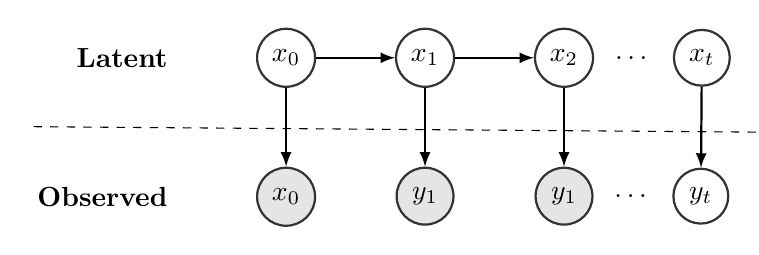
\begin{tikzpicture}
  \def\n{2}
  \node[box,draw=white!100] (Latent) {\textbf{Latent}};

  % Draw base case: x0, y0, and x0 -> y0
  \node[main] (x_0) [right=of Latent] {$x_0$};
  \node[main,fill=black!10] (y_0) [below=of x_0] {$x_0$};
  \path (x_0) edge [connect] (y_0);

  \foreach \i [evaluate = \i as \j using (\i - 1)] in {1,...,\n} {
  	% Draw next cases: x_t, y_t, x{t-1} -> x_t, and x_t -> y_t.
    \node[main] (x_\i) [right=of x_\j] {$x_\i$};
    \node[main,fill=black!10] (y_\i) [below=of x_\i] {$y_1$};
    \path (x_\j) edge [connect] (x_\i);
    \path (x_\i) edge [connect] (y_\i);
  }

  \node[box,draw=white!100,left=of y_0] (Observed) {\textbf{Observed}};

%  Final case: x_t, y_t, x_t -> y_t, and dashed line joining them.
  \node[main] (x_t) [right=of x_\n] {$x_t$};
  \node[main] (y_t) [right=of y_\n] {$y_t$};
  \path (x_t) edge [connect] (y_t);
  \path (x_\n) -- node[auto=false]{\ldots} (x_t);
  \path (y_\n) -- node[auto=false]{\ldots} (y_t);

  % draw the dotted line connecting x_n -> x_t
  \draw [dashed, shorten >=-1cm, shorten <=-1cm]
      ($(Latent)!0.5!(Observed)$) coordinate (a) -- ($(x_t)!(a)!(y_t)$);
\end{tikzpicture}

\vspace{5mm}

The transition density $ p(x_i | x_{i - 1})$ means the system likes to `stick`
in the current state with probability $p$.

\[   
p(x_i | x_{i - 1}) = 
     \begin{cases}
       \text{$p$,} &\quad\text{if  } x_i = x_{i - 1} \\
       \text{$1 - p$,} &\quad\text{otherwise.} \\ 
     \end{cases}
\]

Finally, assume $ X_0 \sim Bernoulli(\frac{1}{2}) $

\end{frame}


%%%%% Generating data with Python %%%%%
\begin{frame}[fragile]{Generating Data with Python (part 1)}
  \begin{figure}
  \centering
      \tiny
   \lstset{language=python,
		basicstyle=\ttfamily,
		keywordstyle=\color{blue}\ttfamily,
		stringstyle=\color{red}\ttfamily,
		commentstyle=\color{green}\ttfamily,
		morecomment=[l][\color{magenta}]{\#}
   }
         \lstinputlisting{code-fragments/simulate_setup.py}
   \end{figure}
\end{frame}

\begin{frame}[fragile]{Generating Data with Python (part 2)}
  \begin{figure}
  \centering
      \tiny
   \lstset{language=python,
		basicstyle=\ttfamily,
		keywordstyle=\color{blue}\ttfamily,
		stringstyle=\color{red}\ttfamily,
		commentstyle=\color{green}\ttfamily,
		morecomment=[l][\color{magenta}]{\#}
   }
         \lstinputlisting{code-fragments/simulate_forward.py}
   \end{figure}
\end{frame}



\begin{frame}{The Bootstrap Particle Filter: Intuition}
Intuition
\end{frame}

\begin{frame}{The Bootstrap Particle Filter: Pseudocode}
\fbox{\parbox{\textwidth}{The Bootstrap Filter
	\begin{enumerate}
		\item \underline{\textit{Initialization}},
			  $t = 0$.
		\begin{itemize}
			\item For $i = 1, ..., N$, sample $\mathbf{x}^{(i)}_0 \sim p(\mathbf{x}_0)$ and set $t = 1$.
		\end{itemize}
	
		\item \underline{\textit{Importance sampling step}}
		\begin{itemize}
			\item For $i = 1, ..., N$, sample
			$\tilde{\mathbf{x}}^{(i)}_t \sim p(\mathbf{x}_t | \mathbf{x}_{t-1}^{(i)})$ 
    	    and set $\tilde{\mathbf{x}}^{(i)}_{0:t} = 
    	    (\mathbf{x}_{0:t - 1}^{(i)}, \tilde{\mathbf{x}}_t^{(i)})$
    	    
    	    \item For $i = 1,..,N$, evaluate the importance weights
         	$$ \tilde{w}^{(i)}_t = p(\mathbf{y}_t | \tilde{\mathbf{x}}_t^{(i)}) $$
         	
         	\item Normalise the importance weights
         	
		\end{itemize}
		
		\item \underline{\textit{Selection Step}}
		\begin{itemize}
			\item Resample with replacement $N$ particles
			$\big(\mathbf{x}_{0:t}^{(i)}; i = 1,...,N\big)$
			from the set
			$\big(\tilde{\mathbf{x}}_{0:t}^{(i)}; i = 1,...,N\big)$
			according to the importance weights.
			
			\item Set $t \gets t + 1$ and go to step 2.
		\end{itemize}
		
	\end{enumerate}
}}

\tiny{
An introduction to Sequential Monte Carlo Methods, (Doucet, de Freitas, Gordon, p 11)
}

\end{frame}

\begin{frame}[fragile]{The Bootstrap Particle Filter: Python implementation}
  \begin{figure}
  \centering
      \tiny
   \lstset{language=python,
		basicstyle=\ttfamily,
		keywordstyle=\color{blue}\ttfamily,
		stringstyle=\color{red}\ttfamily,
		commentstyle=\color{green}\ttfamily,
		morecomment=[l][\color{magenta}]{\#}
   }
         \lstinputlisting{code-fragments/bootstrap.py}
   \end{figure}
\end{frame}



\begin{frame}{Experiments!}

Accuracy metric: \% of times state identified correctly, averaged over $10,000$ runs, for the parameters $ p = 0.95 $, $\mu = 1$, and $N = 1000$ particles.

\vspace{5mm}

\begin{tabular}{ l | c }
  algorithm & accuracy \\
  \hline
  Baseline 	& 69\% \\
  Viterbi 	& 86\% \\
  Bootstrap & 87\% \\
 \end{tabular}

\vspace{5mm}

Minor difference between Viterbi and Bootstrap might be due to metric chosen. Or a bug :-)

It returns MAP estimate - if it estimates state wrong, it can have knock-on effects.

\end{frame}

\begin{frame}{More Experiments!}
Heatmap over grid of $p \in [0.5, 1]$ and $\mu \in [0, 3]$.
Expected outcome: incorporating time series information only matters when $\mu$ is small and $p$ is large.

If $\mu$ is large, then there is little overlap between the two distributions.

If $p$ is close to $0.5$, then each observation is more-or-less independent.
\end{frame}


\end{document}